% Experiments section draft (Section 4 through Experiment 1).
% Self-contained so it compiles standalone; lift the body into the NeurIPS
% paper as needed. The results table uses booktabs, per NeurIPS convention.

\documentclass{article}
\usepackage{booktabs}
\usepackage{graphicx}
\usepackage{amsmath}
\usepackage[margin=1in]{geometry}

\begin{document}

\section{Experiments}

We evaluate our pipeline on the SoccerNet Game State Reconstruction (GSR)
dataset and compare against its official deep-learning baseline. Our
experiments are organized around three questions: is a classical homography
\emph{accurate enough} for minimap localization (Experiment~1), does each
component of the pipeline \emph{earn its place} (Experiment~2), and is the
method \emph{cheap enough} to deliver on its accessibility motivation
(Experiment~3). This draft covers the setup and Experiment~1.

\subsection{Experimental Setup}

\paragraph{Dataset.}
We use the validation split of the SoccerNet GSR dataset: 58 broadcast clips,
each 30 seconds long at 25 frames per second (750 frames of
$1920\times1080$ video), spanning varied stadiums, lighting, and camera work.
Every frame is annotated with pitch-line points and with player, goalkeeper,
referee, and ball bounding boxes, each carrying a ground-truth pitch
coordinate.

\paragraph{Baseline.}
We compare against SoccerNet's \texttt{sn-gamestate} baseline, a deep
multi-stage pipeline whose camera calibration is a trained neural network
producing a full 3D camera model. We obtain its predictions from the official
released baseline tracker state, which provides, for every clip, the
baseline's detected pitch lines, detected boxes, and predicted pitch
positions. We note that the baseline does not place the ball on its 2D
minimap at all: its radar visualization explicitly skips ball detections, and
its detector in any case rarely localizes the ball (e.g.\ producing ball
detections in only 0 and 5 of 750 frames on two inspected clips). In contrast,
our pipeline reconstructs the ball explicitly, including a physics-based
correction for airborne frames.

\paragraph{Inputs and metric.}
Our pipeline consumes only per-frame pitch lines and player/ball detections;
obtaining these is a standard perception problem outside our scope, so we
evaluate our geometry under two input regimes --- the dataset's ground-truth
annotations, and the baseline's own (imperfect) detected lines and boxes. The
latter lets us compare geometry methods on identical inputs. Unless stated
otherwise, error is the Euclidean distance, in metres on the pitch, between a
predicted position and its ground-truth pitch coordinate.

\subsection{Experiment 1: Player Localization Accuracy}

\paragraph{Goal.}
Determine whether a classical planar homography is accurate enough for
minimap localization, and how it compares to the baseline's learned 3D
calibration.

\paragraph{Protocol.}
We measure per-detection localization error for all on-pitch persons across
all 58 validation clips (the ball is excluded here, as its ground-truth pitch
coordinate is unreliable when airborne; the ball is addressed in
Experiment~2), under three conditions:
\begin{itemize}
  \item \textbf{Ours (GT lines)} --- our homography estimated from the
    dataset's ground-truth pitch lines, projecting ground-truth foot points.
    With perfect inputs, this is an upper bound on our geometry.
  \item \textbf{Ours (SoccerNet inputs)} --- our homography estimated from the
    baseline's \emph{detected} pitch lines, projecting the baseline's
    \emph{detected} foot points.
  \item \textbf{SoccerNet} --- the baseline's own predicted positions from its
    3D calibration.
\end{itemize}
The latter two conditions operate on identical detections, so any difference
between them isolates the geometry method. To score the baseline's detections
against ground truth, each detection is matched to a ground-truth box by
greedy image-space IoU (threshold 0.5); unmatched detections are a
perception-recall issue and are excluded.

\paragraph{Results.}
Table~\ref{tab:exp1} reports the error distribution, aggregated over 696{,}776
detections for the ground-truth-input condition and 569{,}075 matched
detections for the two detected-input conditions.

\begin{table}[t]
  \caption{Player localization error against ground truth, over all 58
    validation clips. ``Ours (GT lines)'' uses perfect inputs and is an upper
    bound; the other two conditions share SoccerNet's detections and thus
    isolate the geometry method. Median and p90 are in metres; the last three
    columns are the percentage of detections within the given radius. Best
    per column in bold.}
  \label{tab:exp1}
  \centering
  \begin{tabular}{lccccc}
    \toprule
    Condition & Median (m) & p90 (m) & $<$1\,m (\%) & $<$2\,m (\%) & $<$5\,m (\%) \\
    \midrule
    Ours (GT lines)         & \textbf{0.48} & \textbf{1.78}  & \textbf{78.1} & \textbf{91.2} & \textbf{96.8} \\
    Ours (SoccerNet inputs) & 0.84          & 3.60           & 57.6          & 80.3          & 93.0 \\
    SoccerNet               & 0.98          & 20.22          & 50.7          & 69.7          & 78.9 \\
    \bottomrule
  \end{tabular}
\end{table}

With ground-truth lines our homography localizes players to a median of
0.48\,m, with 91\% of detections within 2\,m. Fed the baseline's own detected
lines and boxes --- a controlled, like-for-like test of geometry --- our
method achieves a median error of 0.84\,m, \emph{lower} than the baseline's
0.98\,m on the identical detections, and wins at every tolerance (e.g.\ 80.3\%
vs.\ 69.7\% within 2\,m). The gap is most pronounced in the tail: our
90th-percentile error is 3.60\,m, against 20.22\,m for the baseline --- one in
ten of the baseline's predictions is off by more than 20\,m. The mean error is
the lone metric favouring the baseline (7.90\,m vs.\ our 8.70\,m); this
statistic is dominated by a thin tail of extreme frames --- our method in fact
produces \emph{fewer} large errors (7\% beyond 5\,m vs.\ the baseline's 21\%)
--- so we report the robust median and threshold fractions as the primary
measures.

Figure~\ref{fig:exp1} shows a representative frame. Our reconstruction, under
both input regimes, reproduces the ground-truth player configuration, whereas
the baseline's calibration shifts the entire formation by roughly 15\,m. The
$0.48 \rightarrow 0.84$\,m increase between our two input regimes quantifies
the cost of imperfect detected lines.

\begin{figure}[t]
  \centering
  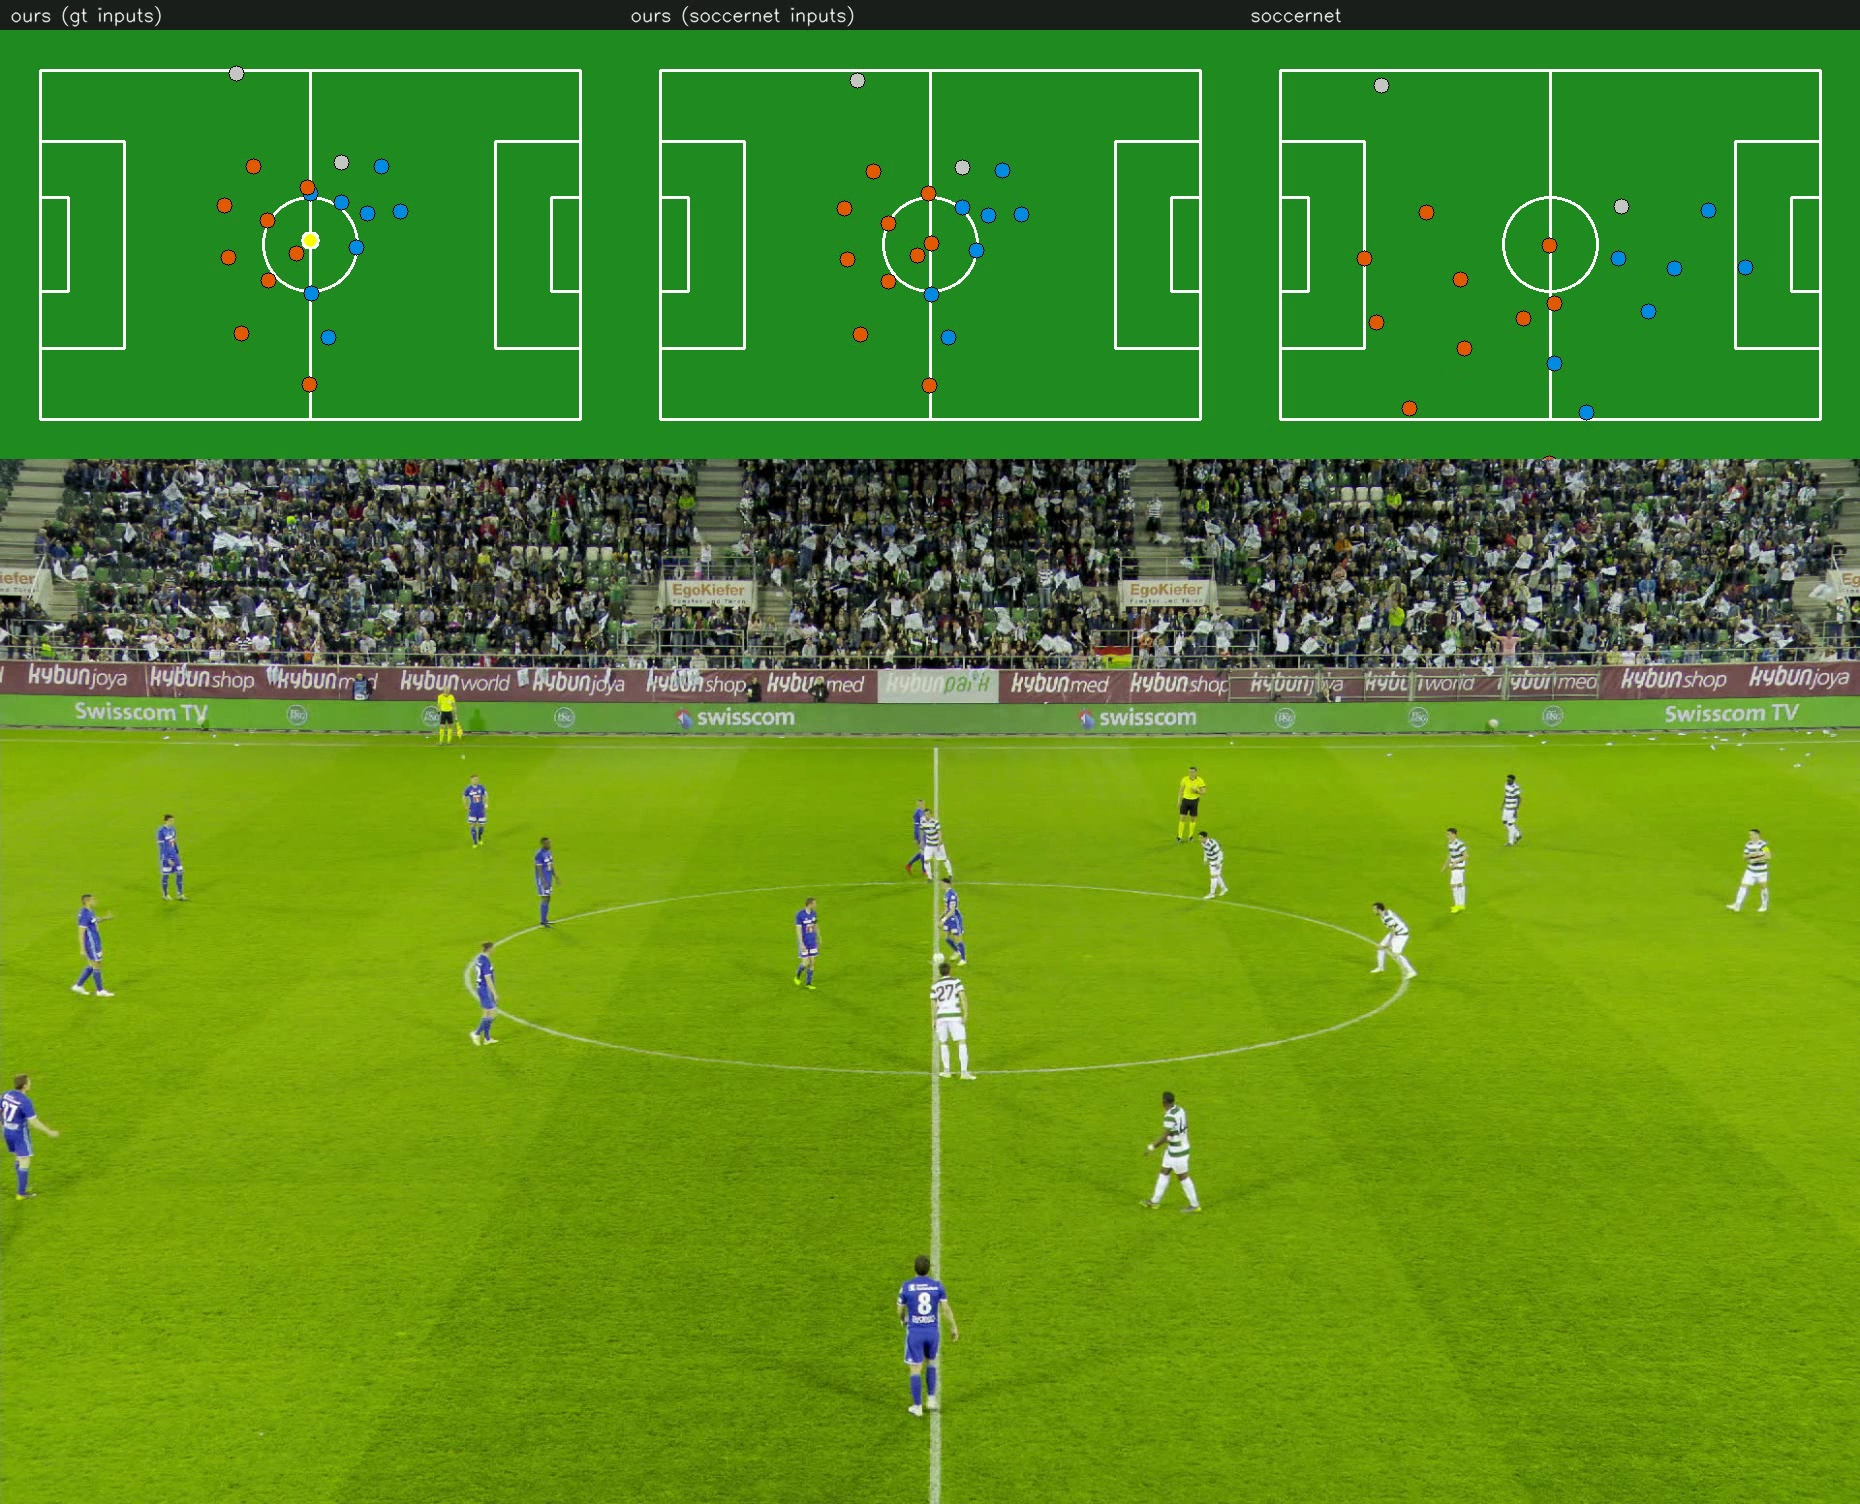
\includegraphics[width=\textwidth]{outputs/SNGS-095/experiment1_figure.jpg}
  \caption{Localization on clip SNGS-095 (an illustrative example; the full
    distribution is in Table~\ref{tab:exp1}). Top, left to right: minimaps from
    our homography on ground-truth inputs, our homography on SoccerNet's
    detected inputs, and SoccerNet's own 3D calibration. Bottom: the source
    broadcast frame. Both of our reconstructions match the true formation; the
    baseline displaces it by ${\sim}15$\,m. The ball (yellow) appears only in
    our ground-truth-input panel: our pipeline reconstructs it, whereas the
    SoccerNet baseline neither reliably detects the ball nor places it on the
    minimap.}
  \label{fig:exp1}
\end{figure}

\paragraph{Takeaway.}
A classical planar homography matches and, on this evidence, exceeds a trained
3D-calibration network for minimap player localization, while requiring no
training, no learned weights, and no GPU.

\subsection{Experiment 2: Component Ablation}

\paragraph{Goal.}
Our pipeline adds three components on top of a plain homography fit:
circle-based handling of degenerate camera views, temporal smoothing, and
physics-based gating of the airborne ball. We disable each in turn and measure
the metric it targets, over all 58 clips (43{,}500 frames), to confirm each
earns its place. Results are summarized in Table~\ref{tab:exp2}.

\paragraph{Circle-degeneracy handling.}
Many broadcast frames show only mutually parallel pitch lines --- for example
the two sidelines and the halfway line --- which cannot constrain an
eight-degree-of-freedom homography. For these frames our method adds point
correspondences derived from the central circle. With this component disabled,
the fraction of frames yielding a valid homography falls from 96.3\% to
81.6\%: circle handling recovers 14.7\% of all frames (roughly 6{,}400 frames)
that would otherwise have no minimap at all.

\paragraph{Temporal smoothing.}
Independently fitted homographies jitter from frame to frame. We measure the
per-frame displacement of fixed probe points projected onto the pitch; as this
quantity is heavy-tailed (a failed fit sends probe points near-infinitely
far), we report the median and tail percentiles. The median-filter smoothing
reduces the 90th-percentile displacement from 3.90\,m to 2.89\,m and the 95th
from 12.79\,m to 9.06\,m ($-26\%$ / $-29\%$), and the rate of large
($>$5\,m) frame-to-frame jumps from 8.7\% to 7.2\%, while leaving the median
essentially unchanged (0.37\,m $\rightarrow$ 0.31\,m). It thus suppresses
jitter without lagging genuine camera motion.

\paragraph{Airborne-ball gating.}
A ground-plane homography cannot localize an airborne ball: its image point
can back-project far off the pitch. Without gating, the raw ball projection
lands off the pitch in 3{,}895 frames; our physics-based gate and trajectory
interpolation reduce this to zero. On frames where the ball's ground-truth
position is itself reliable, gating leaves accuracy unchanged (median error
$0.63 \rightarrow 0.64$\,m, mean $1.68 \rightarrow 1.59$\,m) --- it eliminates
the catastrophic frames at no cost to the rest.

\begin{table}[t]
  \caption{Component ablation over all 58 validation clips (43{,}500 frames).
    Each component is disabled in turn and evaluated by the metric it targets.
    ``Full'' is the complete pipeline; ``Ablated'' removes that one component.}
  \label{tab:exp2}
  \centering
  \begin{tabular}{llcc}
    \toprule
    Component ablated & Metric & Full & Ablated \\
    \midrule
    Circle-degeneracy handling & Frames with valid homography (\%) & \textbf{96.3} & 81.6 \\
    Temporal smoothing         & p95 probe displacement (m)        & \textbf{9.06} & 12.79 \\
    Airborne-ball gating       & Off-pitch ball frames             & \textbf{0}    & 3895 \\
    \bottomrule
  \end{tabular}
\end{table}

\paragraph{Takeaway.}
All three components yield measurable improvements: circle handling and ball
gating eliminate outright failures (unsolvable frames and off-pitch ball
projections), while temporal smoothing reduces residual jitter without
sacrificing responsiveness to real camera motion.

\end{document}
